%!TEX root = ../thesis.tex

\section{性能評価の方法}
本章では，提案手法の基本的な性能を明らかにするための評価実験について述べる．この実験の目的は，従来手法と比較して提案手法がどの程度処理速度を向上させるか，またその際にどの程度の検出位置の正確度を維持できるかを定量的に評価することである．
実験環境の詳細を\Table{tab:env_evaluation}に示す．コンピュータは後述のモビリティの制御に用いる NVIDIA Jetson AGX Orin (32GB) を使用し，MOT17データセット\cite{ref9}を使用した．また，テキストプロンプトには“pedestrian”を指定した．

\begin{table}[htbp]
\centering
\caption{Experimental environment for evaluation}
\label{tab:env_evaluation}
\begin{tabular}{ll}
\hline
Computer & NVIDIA Jetson AGX Orin 32GB \\
Input Text & "pedestrian." \\
Grounding DINO & grounding-dino-base \\
SAM Model & sam2.1\_hiera\_small \\
\hline
\end{tabular}
\end{table}

\newpage

\section{結果と考察}
評価指標には，システム全体の処理速度を示す FPS (Frames Per Second) と，BBoxの正確度を示す IoU (Intersection over Union) の2つを用いた．評価データには，mot17-02-frcnnの 600 フレームを用いた．比較対象として，毎フレーム物体検出を行う従来手法（Lang-SAM）でも同様の評価を行った．

実験結果を\Table{tab:results}に示す．提案手法は従来手法に比べて処理速度を向上させる一方で，正確度の低下も確認された．この結果は，本手法において処理速度と正確度がトレードオフの関係にあることを示している．検出結果の一例を\Fig{fig:results}に示す．図中では，正解データを赤色で，従来手法を青色で，提案手法を緑色で示している．図のように，完全一致ではないものの，提案手法により歩行者を概ね正しく検出できていることがわかる．

\begin{table}[htbp]
\centering
\caption{Experimental results for evaluation}
\label{tab:results}
\begin{tabular}{lcccc}
\hline
Method & FPS & IoU \\
\hline
Conventional & 0.79 & 0.814 \\
Proposed (Redetection interval: 2.0s) & 2.15 & 0.707 \\
\hline
\end{tabular}
\end{table}

\begin{figure}[H]
\centering
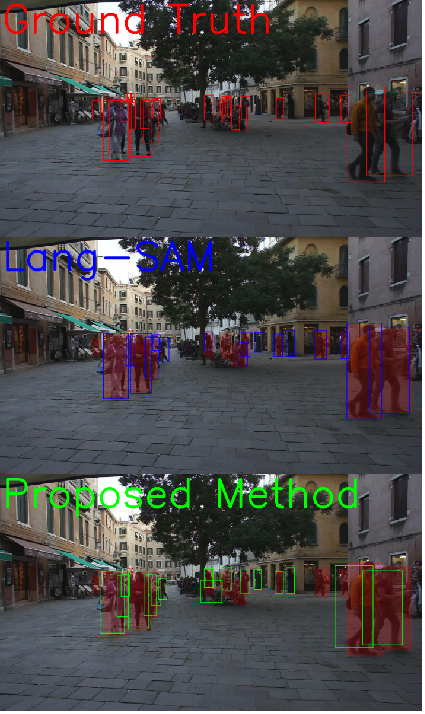
\includegraphics[width=0.85\linewidth]{images/pdf/evaluation.pdf}
\caption{Comparison of Ground Truth, Lang-SAM, and the Proposed Method}
\label{fig:results}
\end{figure}

\newpage
